\section{初值与边界数据}
\label{sec:pdeprob-data}

方程只规定区域内部每一点上的局部关系，它本身确定不了解。仍以$(0,1)$上的细棒为例，下面几个函数都满足$\partial_tu=\partial_x^{2}u$：
\[
  u=0,\qquad u=x,\qquad u=x^{2}+2t,\qquad u=\mathrm{e}^{-\pi^{2}t}\sin\pi x.
\]
第三个函数的两个偏导数都是$2$；第四个函数的两个偏导数都等于$-\pi^{2}\mathrm{e}^{-\pi^{2}t}\sin\pi x$。

缺少的信息有多少？一阶常微分方程的通解含一个任意常数，补一个初值就够了。偏微分方程的通解含任意函数。例如$\partial_tu+\partial_xu=0$的解可以写成$u=\varphi(x-t)$，其中$\varphi$是任意可微函数，由链式法则，$\partial_tu=-\varphi'$，$\partial_xu=\varphi'$，两者相加为零。所以需要补充的也是函数，它们定义在比时空低一维的集合上：初始时刻的切片和区域的边界。

演化问题的自变量落在\term{时空柱}（space-time cylinder）$Q=\Omega\times(0,T)$中。图~\ref{fig:pdeprob-cylinder}画出它的三块边界：底面是初始时刻，侧面是空间边界随时间展开，顶面是终止时刻。以热方程为例，典型的问题是
\begin{equation}
  \begin{cases}
    \partial_tu-\Delta u=f & \text{在}\ Q\ \text{内},\\
    u=g & \text{在}\ \partial\Omega\times(0,T)\ \text{上},\\
    u(\cdot,0)=u_0 & \text{在}\ \Omega\ \text{上}.
  \end{cases}
  \label{eq:pdeprob-heat-ibvp}
\end{equation}

\begin{BookInlineFigure}
  \centering
  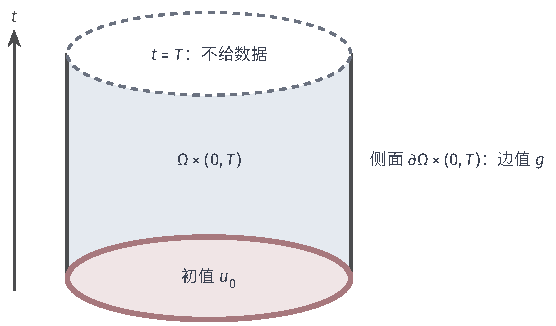
\includegraphics[width=94.1mm]{figures/06-differential-equations/02-partial-differential-equations/tikz/pdeprob-cylinder/figure.pdf}
  \caption{时空柱$Q=\Omega\times(0,T)$。红色底面给初值，深灰色侧面给边值，虚线所示的顶面$t=T$不给数据，那里的值由演化决定。}
  \label{fig:pdeprob-cylinder}
\end{BookInlineFigure}

数据的个数和位置不是随意的，还要与方程传播信息的方式相合。热方程不在顶面给数据，输运方程只在一部分侧面给数据，波动方程在底面要给两个函数。下面分三部分讨论：初始状态要给几个函数、边界上能给什么、两者交接时要满足什么。

\subsection{初始数据}
\label{sec:pdeprob-initial}

为什么热方程只要一个初值，而波动方程要两个？比较这两个方程在$t=0$能告诉我们什么。

\paragraph{时间阶数与初始状态}
在$(0,1)$上给定初始温度$u_0$，且两端为零。热方程的右端可以由$u_0$算出，于是$\partial_tu(\cdot,0)=\partial_x^{2}u_0$，时间一阶导数已经由方程确定，不必再给。

波动方程不同。给定初始位移$u_0$，方程只确定了$\partial_t^{2}u(\cdot,0)=c^{2}\partial_x^{2}u_0$，时间一阶导数还是自由的。这和常微分方程$\ddot{x}=-x$必须同时给位置和速度是一回事，只是位置和速度现在都是函数。所以波动方程的初始状态是一对函数：
\begin{equation}
  u(\cdot,0)=u_0,\qquad \partial_tu(\cdot,0)=u_1.
  \label{eq:pdeprob-wave-initial}
\end{equation}

下面取$c=1$、两端固定，给定同一个初始位移$u_0=\sin\pi x$，算两个不同的解。直接代入可以验证，下面两个函数都满足波动方程和零边值，且在$t=0$的位移都是$\sin\pi x$：
\[
  u^{\mathrm{a}}=\cos(\pi t)\sin\pi x,\qquad
  u^{\mathrm{b}}=\bigl(\cos(\pi t)+\sin(\pi t)\bigr)\sin\pi x.
\]
区别在初始速度：$\partial_tu^{\mathrm{a}}(x,0)=0$，而$\partial_tu^{\mathrm{b}}(x,0)=\pi\sin\pi x$。

图~\ref{fig:pdeprob-wave-velocity}(b)比较弦中点的历史。两条波动曲线从同一点出发，随后分开，所以只给位移不能确定解。同样的初值在热方程下只有一条曲线，就是$\mathrm{e}^{-\pi^{2}t}$，第~\ref{sec:pdeprob-well-posedness}节将证明它是唯一的。

\begin{BookInlineFigure}
  \centering
  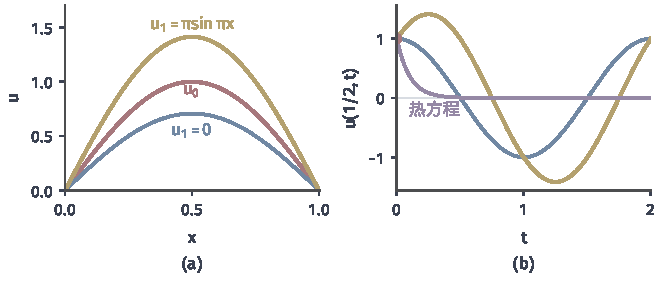
\includegraphics[width=112.0mm]{figures/06-differential-equations/02-partial-differential-equations/matplotlib/pdeprob-wave-velocity/figure.pdf}
  \caption{同一初始位移$u_0=\sin\pi x$（红），$c=1$。(a)$t=1/4$时的弦形：初速度为零（蓝）和初速度为$\pi\sin\pi x$（黄）。(b)中点$x=1/2$的时间历史，蓝、黄同(a)，紫线是热方程在同一初值下的解。}
  \label{fig:pdeprob-wave-velocity}
\end{BookInlineFigure}

一般地，若方程能解出最高阶时间导数，即$\partial_t^{k}u$可以用较低阶时间导数和空间导数表示，就需要$k$个初始函数。这时可以逐阶求出$t=0$处的全部时间导数。以波动方程的$u^{\mathrm{b}}$为例，由初始数据得$\partial_t^{2}u=-\pi^{2}\sin\pi x$，对方程再求一次时间导数得$\partial_t^{3}u=-\pi^{3}\sin\pi x$，这正是$u^{\mathrm{b}}$的Taylor系数。

这个计数只是必要的预期，不保证问题可解。第~\ref{sec:pdeprob-well-posedness}节会看到，把Laplace方程中的一个空间变量当成“时间”，也可以解出二阶导数并给两个初始函数，结果却完全不可用。

\paragraph{初值的光滑程度}
初值的光滑程度决定方程在初始时刻能否按经典意义解释。取折线初值
\begin{equation}
  u_0(x)=\min\{x,1-x\},
  \label{eq:pdeprob-hat}
\end{equation}
它在$x=1/2$处没有导数，$\partial_x^{2}u_0$不存在，所以方程在$t=0$的这一点上没有意义。解决办法是只要求方程在$t>0$成立，初值作为$t\to0$时的极限取到。

这样解释后，热方程和波动方程的表现完全不同。把$u_0$展开成正弦级数，系数为
\[
  b_k=2\int_0^{1}u_0(x)\sin(k\pi x)\,\mathrm{d}x=\frac{4\sin(k\pi/2)}{k^{2}\pi^{2}},
\]
热方程的解和$c=1$的波动方程在初速度为零时的解分别是
\[
  \sum_{k\geq1}b_k\mathrm{e}^{-k^{2}\pi^{2}t}\sin k\pi x,\qquad
  \sum_{k\geq1}b_k\cos(k\pi t)\sin k\pi x.
\]

对热方程，每求一次$x$的导数系数多一个因子$k\pi$，但只要$t>0$，因子$\mathrm{e}^{-k^{2}\pi^{2}t}$比任何多项式衰减得都快，求导后的级数仍然收敛，解立即变得光滑。在$t=0$，二阶导数的级数通项是$-4\sin(k\pi/2)\sin(k\pi x)$，不趋于零，这正对应$\partial_x^{2}u_0$不存在。

对波动方程，系数没有衰减因子。解等于$\frac12[u_0^{*}(x-t)+u_0^{*}(x+t)]$，其中$u_0^{*}$是$u_0$在实轴上的奇周期延拓。折角被原样带着走，分成两个折角向两边移动。图~\ref{fig:pdeprob-kink-heat-wave}对比了两种情形：(a)的折角瞬间变圆，(b)的折角一直保持。所以波动方程在$t>0$时沿这两条线仍不能按经典意义解释；这样的函数算不算解，要到第~\ref{sec:pdeprob-solutions}节再回答。

\begin{BookInlineFigure}
  \centering
  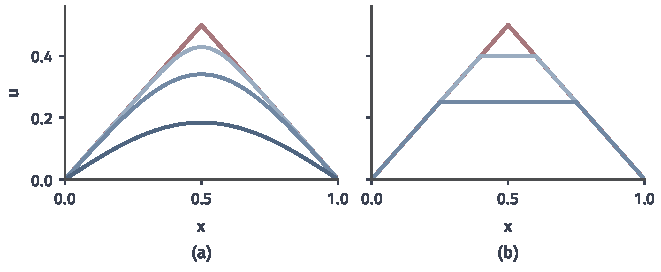
\includegraphics[width=112.0mm]{figures/06-differential-equations/02-partial-differential-equations/matplotlib/pdeprob-kink-heat-wave/figure.pdf}
  \caption{折线初值$u_0=\min\{x,1-x\}$（红），两端为零。(a)热方程，蓝色由浅到深为$t=0.004,0.02,0.08$，折角立即消失（$600$项正弦级数）。(b)波动方程，$c=1$，初速度为零，蓝色由浅到深为$t=0.1,0.25$，两个折角分别向左右移动，中间是一段平台。}
  \label{fig:pdeprob-kink-heat-wave}
\end{BookInlineFigure}

\subsection{边界数据}
\label{sec:pdeprob-boundary}

区域有边界，边界上发生的事也要交代。边界条件规定的可以是场值，可以是穿过边界的通量，也可以是两者之间的关系。

\paragraph{三类边界条件}
记$\partial_{\bm{n}}u=\nabla u\cdot\bm{n}$，它是$u$沿离开区域方向的变化率，称为\term{法向导数}（normal derivative）。按照热传导的语言，$\partial\Omega$上常见的条件是：
\begin{align}
  u&=g, \label{eq:pdeprob-dirichlet}\\
  \partial_{\bm{n}}u&=g, \label{eq:pdeprob-neumann}\\
  \partial_{\bm{n}}u+\alpha u&=g. \label{eq:pdeprob-robin}
\end{align}
依次称为\term{Dirichlet边界条件}（Dirichlet boundary condition）、\term{Neumann边界条件}（Neumann boundary condition）和\term{Robin边界条件}（Robin boundary condition）。

Dirichlet条件直接规定温度，如棒端浸在恒温水中。Neumann条件规定穿过边界的通量，向外的热流是$-\partial_{\bm{n}}u$，所以$g=0$表示绝热。Robin条件来自Newton冷却定律：向外的热流正比于边界温度与环境温度$u_{\mathrm{env}}$之差，$-\partial_{\bm{n}}u=\alpha(u-u_{\mathrm{env}})$，整理后就是式~\eqref{eq:pdeprob-robin}，其中$g=\alpha u_{\mathrm{env}}$。

物理上$\alpha\geq0$。$\alpha<0$意味着边界越热吸收得越多，这种正反馈下后面的估计不再成立。系数不是单位矩阵时，通量是$\bm{A}\nabla u$，法向导数相应换成$\bm{n}^{\top}\bm{A}\nabla u$。不同边界段可以使用不同类型，如图~\ref{fig:pdeprob-boundary-types}。

\begin{BookInlineFigure}
  \centering
  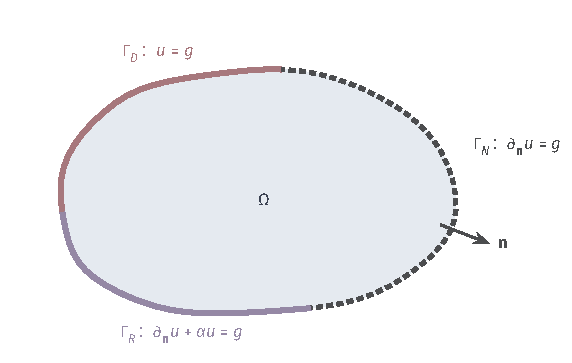
\includegraphics[width=96.9mm]{figures/06-differential-equations/02-partial-differential-equations/tikz/pdeprob-boundary-types/figure.pdf}
  \caption{同一区域的边界分成三段：红色段$\Gamma_D$规定场值，深灰虚线段$\Gamma_N$规定法向导数，紫色段$\Gamma_R$规定场值和法向导数的组合。$\bm{n}$是单位外法向。}
  \label{fig:pdeprob-boundary-types}
\end{BookInlineFigure}

边界类型会改变解本身。下面在$(0,1)$上取方程$-u''=2$和右端条件$u(1)=0$，通解是
\[
  u(x)=-x^{2}+Ax+B.
\]
左端点的外法向指向$-x$方向，所以左端的$\partial_{\bm{n}}u=-u'(0)$。下面依次取三种条件。

Dirichlet条件$u(0)=0$给出$B=0$，再由$u(1)=0$得$A=1$，于是
\[
  u(x)=x(1-x),\qquad \max_xu=\frac14.
\]

Neumann条件$u'(0)=0$给出$A=0$，再由$u(1)=0$得$B=1$，于是
\[
  u(x)=1-x^{2},\qquad \max_xu=1.
\]

Robin条件取$\alpha=1$、$g=0$，即$-u'(0)+u(0)=0$，给出$A=B$。再由$u(1)=-1+2B=0$得$B=1/2$，于是
\[
  u(x)=\frac12+\frac12x-x^{2},\qquad \max_xu=u\Bigl(\frac14\Bigr)=\frac{9}{16}.
\]

图~\ref{fig:pdeprob-bc-solutions}中，三条曲线的热源和右端相同，只有左端不同：Dirichlet曲线被钉在零，Neumann曲线的切线水平，Robin曲线的切线斜率等于端点值$1/2$。左端越容易散热，整根棒越凉：Dirichlet、Robin、Neumann三种情形的最高温依次是$1/4$、$9/16$、$1$。

\begin{BookInlineFigure}
  \centering
  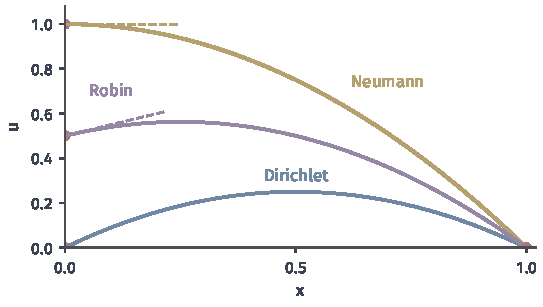
\includegraphics[width=92.0mm]{figures/06-differential-equations/02-partial-differential-equations/matplotlib/pdeprob-bc-solutions/figure.pdf}
  \caption{$-u''=2$、$u(1)=0$在三种左端条件下的解。红点是端点值，虚线是左端切线。}
  \label{fig:pdeprob-bc-solutions}
\end{BookInlineFigure}

\paragraph{输运方程的入流边界}
对$\Omega$的整个边界都规定数据，在二阶椭圆方程中是合理的，在输运方程中却不行。想象水流搬运墨水：墨水的浓度由上游决定，下游端点流出的是已经确定的东西，不能再规定。

在$(0,1)$上取$v=1$，方程$\partial_tu+\partial_xu=0$的信息沿直线$x=x_0+t$传递。设$u(\cdot,0)=u_0$，左端$u(0,t)=g(t)$，沿着这些路径回溯，解是
\begin{equation}
  u(x,t)=\begin{cases}u_0(x-t),&x>t,\\ g(t-x),&x<t.\end{cases}
  \label{eq:pdeprob-transport-solution}
\end{equation}
右端的值$u(1,t)$已经由式~\eqref{eq:pdeprob-transport-solution}确定。若再独立规定$u(1,t)=h(t)$，除非$h$恰好等于算出来的值，否则问题无解。

一般地，定义\term{入流边界}（inflow boundary）和\term{出流边界}（outflow boundary）为
\begin{equation}
  \Gamma_{-}=\{\bm{x}\in\partial\Omega:\bm{v}\cdot\bm{n}<0\},\qquad
  \Gamma_{+}=\{\bm{x}\in\partial\Omega:\bm{v}\cdot\bm{n}>0\}.
  \label{eq:pdeprob-inflow}
\end{equation}
$\bm{v}\cdot\bm{n}<0$表示流动指向区域内部，边界数据只在$\Gamma_{-}$上给出；$\bm{v}$随时间变化时，这两部分也随时间变化。入流边界的位置由速度场决定，而不是由几何形状决定。

图~\ref{fig:pdeprob-inflow}画出区间上的三个速度场。(a)$v=1$，只有左端入流。(b)$v=x-1/2$，两端的外法向分别与速度同向，都是出流，因此端点不需要任何数据，解完全由初值决定。(c)$v=1/2-x$，两端都是入流，都要给数据。

\begin{BookInlineFigure}
  \centering
  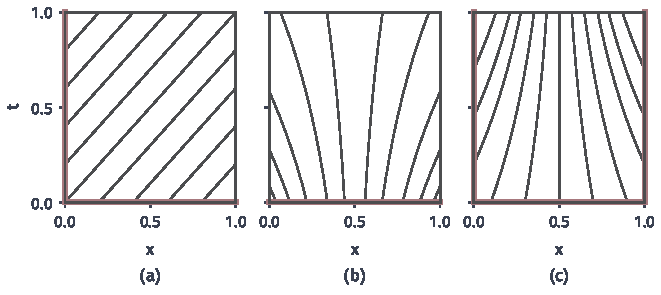
\includegraphics[width=112.0mm]{figures/06-differential-equations/02-partial-differential-equations/matplotlib/pdeprob-inflow/figure.pdf}
  \caption{区间$(0,1)$上三个速度场的粒子路径$\mathrm{d}x/\mathrm{d}t=v$（深灰），红色粗线是需要给数据的边界。(a)$v=1$。(b)$v=x-\frac12$，两端都是出流。(c)$v=\frac12-x$，两端都是入流。每条路径都从红线出发。}
  \label{fig:pdeprob-inflow}
\end{BookInlineFigure}

只在入流边界给数据为什么足够？设$\nabla\cdot\bm{v}=0$，$u$是光滑解，$f=0$。将方程乘以$u$并在$\Omega$上积分。由$\nabla\cdot\bm{v}=0$，对流项可以写成散度：
\[
  u\,\bm{v}\cdot\nabla u=\frac12\nabla\cdot(\bm{v}u^{2}).
\]
再由散度定理，得到
\begin{equation}
  \frac{\mathrm{d}}{\mathrm{d}t}\frac12\int_\Omega u^{2}\,\mathrm{d}\bm{x}
  =-\frac12\int_{\partial\Omega}(\bm{v}\cdot\bm{n})\,u^{2}\,\mathrm{d}S.
  \label{eq:pdeprob-transport-energy}
\end{equation}
出流边界上$\bm{v}\cdot\bm{n}>0$，这一项只会减少能量，不需要控制；入流边界上这一项会增加能量，必须由数据控制。若两个解的初值相同、入流数据相同，它们之差$w$满足式~\eqref{eq:pdeprob-transport-energy}，且$\Gamma_{-}$上$w=0$，所以$\int_\Omega w^{2}$不增，从零出发恒为零。入流数据恰好足以确定解。

\subsection{数据相容性}
\label{sec:pdeprob-compatibility}

初值和边值是分别给出的，但它们在角点处相遇；有些问题的数据之间还有整体的约束。给的数据多，并不意味着有解。

\paragraph{角点处的相容条件}
回到$(0,1)$上的细棒。若初始温度处处为$1$，两端却保持为$0$，那么在角点$(x,t)=(0,0)$附近，沿$t=0$趋近得到$1$，沿$x=0$趋近得到$0$，解不可能在角点连续。

要让解在$\overline{Q}$上连续，需要初值在边界上的取值和边值在初始时刻一致，即零阶\term{相容条件}（compatibility condition）：
\begin{equation}
  u_0(\bm{x})=g(\bm{x},0),\qquad \bm{x}\in\partial\Omega.
  \label{eq:pdeprob-compat-zero}
\end{equation}

要求解更光滑时条件也更多。假设$u$在角点附近有连续的$\partial_tu$和$\partial_x^{2}u$，在左端$x=0$上有$u(0,t)=g(t)$，对$t$求导得$\partial_tu(0,t)=g'(t)$。令$t\to0$，再利用热方程$\partial_tu=\partial_x^{2}u+f$，就得到一阶相容条件：
\begin{equation}
  g'(0)=u_0''(0)+f(0,0).
  \label{eq:pdeprob-compat-one}
\end{equation}
式~\eqref{eq:pdeprob-compat-one}不是额外的物理假设，只是方程在角点处的推论。若要求解有更高阶的连续导数，同样的步骤可以继续，每多要求一阶时间导数，就多一个条件。波动方程的情形类似，表~\ref{tab:pdeprob-compatibility}列出左端点的前几个条件，其中$g$是左端的边值。

\begin{BookInlineTable}
  \centering
  \begin{tabular}{lll}
    \toprule
    方程 & 希望连续到角点的量 & 相容条件\\
    \midrule
    热方程 & $u$ & $u_0(0)=g(0)$\\
    热方程 & $u,\partial_tu,\partial_x^{2}u$ & 另加$g'(0)=u_0''(0)+f(0,0)$\\
    波动方程 & $u$ & $u_0(0)=g(0)$\\
    波动方程 & $u,\partial_tu$ & 另加$u_1(0)=g'(0)$\\
    波动方程 & 全部二阶导数 & 另加$g''(0)=c^{2}u_0''(0)+f(0,0)$\\
    \bottomrule
  \end{tabular}
  \caption{角点处的相容条件随所要求的光滑程度增加。}
  \label{tab:pdeprob-compatibility}
\end{BookInlineTable}

相容条件不满足时，问题不一定无解，而是解的光滑性受限，受限的方式随方程而不同。图~\ref{fig:pdeprob-corner-mismatch}比较初值为$1$、边值为$0$时的两种情形。(a)热方程的解在$t>0$时光滑，不连续性只局限在角点。(b)输运方程的解由式~\eqref{eq:pdeprob-transport-solution}给出，在直线$x=t$左侧为$0$、右侧为$1$，角点处的矛盾被带进区域内部，变成一条持续的间断线。

\begin{BookInlineFigure}
  \centering
  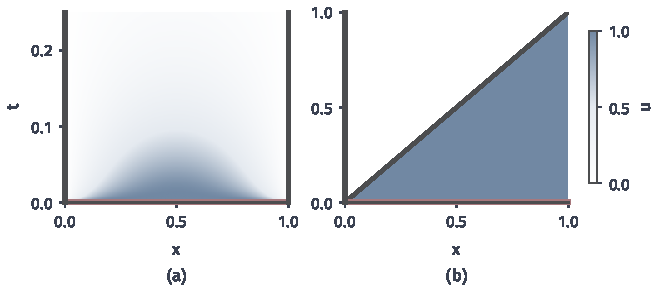
\includegraphics[width=112.0mm]{figures/06-differential-equations/02-partial-differential-equations/matplotlib/pdeprob-corner-mismatch/figure.pdf}
  \caption{初值$u_0=1$（红线）与边值$0$（深灰竖线）不相容。颜色表示$u$的值。(a)热方程，由奇数项正弦级数$\sum_{k}\frac{4}{k\pi}\mathrm{e}^{-k^2\pi^2t}\sin k\pi x$计算。(b)输运方程$v=1$，深灰斜线是间断线$x=t$。两图的时间范围不同。}
  \label{fig:pdeprob-corner-mismatch}
\end{BookInlineFigure}

\paragraph{整体的积分约束}
相容不只发生在角点。考虑Poisson方程配Neumann条件：
\begin{equation}
  -\Delta u=f\ \ \text{在}\ \Omega\ \text{内},\qquad
  \partial_{\bm{n}}u=g\ \ \text{在}\ \partial\Omega\ \text{上},
  \label{eq:pdeprob-neumann-problem}
\end{equation}
其中$\Omega$有界，边界足够规则。把方程在$\Omega$上积分，由散度定理，
\[
  \int_\Omega\Delta u\,\mathrm{d}\bm{x}=\int_{\partial\Omega}\partial_{\bm{n}}u\,\mathrm{d}S.
\]
于是若解存在，数据必须满足
\begin{equation}
  \int_\Omega f\,\mathrm{d}\bm{x}+\int_{\partial\Omega}g\,\mathrm{d}S=0.
  \label{eq:pdeprob-neumann-compat}
\end{equation}

这个条件的含义是收支平衡。$\int f$是内部的总产热，$\int g=\int\partial_{\bm{n}}u$是从外部流入的总热量，平衡状态要求两者之和为零。一个绝热的棒内部持续加热，不可能达到稳态。

在$(0,1)$上取$f=1$、两端绝热$u'(0)=u'(1)=0$。式~\eqref{eq:pdeprob-neumann-compat}左边是$1\neq0$，方程$-u''=1$无解。对应的演化问题$\partial_tu=\partial_x^{2}u+1$却有解，例如从$u_0=\frac12\cos\pi x$出发，
\[
  u(x,t)=t+\frac12\mathrm{e}^{-\pi^{2}t}\cos\pi x.
\]
图~\ref{fig:pdeprob-neumann-balance}(a)中，形状的起伏很快消失，而整体温度以速度$1$不断上升，没有稳态可趋近。

现在改为边界散热，取$u'(0)=1/2$，$u'(1)=-1/2$。这时$\partial_{\bm{n}}u$在两端都是$-1/2$，式~\eqref{eq:pdeprob-neumann-compat}左边是$1-\frac12-\frac12=0$。逐次积分得到解
\[
  u(x)=-\frac{x^{2}}{2}+\frac{x}{2}+C,
\]
其中$C$是任意常数，如图~\ref{fig:pdeprob-neumann-balance}(b)。约束满足了，解却不唯一：方程和边界条件都只含$u$的导数，看不到整体平移。

\begin{BookInlineFigure}
  \centering
  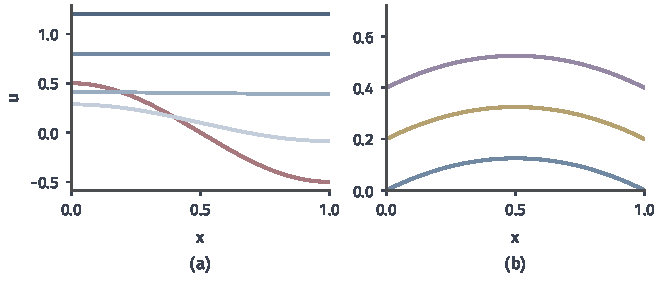
\includegraphics[width=112.0mm]{figures/06-differential-equations/02-partial-differential-equations/matplotlib/pdeprob-neumann-balance/figure.pdf}
  \caption{Neumann问题的积分约束。(a)绝热棒内持续加热，初值（红）的起伏消失，整体上升，蓝色由浅到深为$t=0.1,0.4,0.8,1.2$。(b)加热与散热平衡时$-u''=1$的解$-x^2/2+x/2+C$，$C=0,0.2,0.4$，彼此只差常数。}
  \label{fig:pdeprob-neumann-balance}
\end{BookInlineFigure}

这和线性方程组完全相同。把棒分成三段，每段写热量收支，绝热端没有通量，得到系数矩阵
\[
  \bm{B}=\begin{pmatrix}1&-1&0\\-1&2&-1\\0&-1&1\end{pmatrix},
  \qquad \bm{B}\bm{1}=\bm{0},\qquad \bm{1}^{\top}\bm{B}=\bm{0}^{\top},
\]
其中$\bm{1}=(1,1,1)^{\top}$。方程$\bm{B}\bm{u}=\bm{b}$有解当且仅当$\bm{1}^{\top}\bm{b}=0$，有解时解差$\bm{1}$的倍数。积分约束对应对$\bm{1}$的正交条件，任意常数对应零空间。

这些例子说明，不能靠增加数据的数量来保证有解。数据太少时解不唯一，例如区间上$-u''=f$只给一个端点；数据太多时互相冲突，例如输运方程同时规定两端；个数恰好，也可能违反积分约束。判断的依据是方程的传播方式和结构，下一节把这件事说清楚。
